%% LyX 2.3.4.3 created this file.  For more info, see http://www.lyx.org/.
%% Do not edit unless you really know what you are doing.
\documentclass[english]{article}
\usepackage[T1]{fontenc}
\usepackage[utf8]{inputenc}
\usepackage{geometry}
\geometry{verbose,tmargin=2cm,bmargin=2cm,lmargin=2cm,rmargin=2cm}
\usepackage{babel}
\usepackage{float}
\usepackage{amsmath}
\usepackage{amssymb}
\usepackage{graphicx}
\usepackage{setspace}
\doublespacing
\usepackage[unicode=true]
 {hyperref}

\makeatletter
%%%%%%%%%%%%%%%%%%%%%%%%%%%%%% User specified LaTeX commands.
\usepackage{indentfirst}
\usepackage{mathtools}
\usepackage{listings}
\usepackage{tikz}
\usetikzlibrary{shapes.geometric, arrows}

\tikzstyle{startstop} = [rectangle, rounded corners, minimum width=3cm, minimum height=1cm,text centered, draw=black]
\tikzstyle{io} =        [trapezium, trapezium left angle=85, trapezium right angle=95, minimum width=1cm, minimum height=1cm, text centered, draw=black]
\tikzstyle{arrow} = [thick,->,>=stealth]

\makeatother

\begin{document}
\title{Finding rare trajectories in transiently chaotic systems}
\author{Leonardo L. D. L. Hügens\\
J. M. Viana Parente Lopes\\
Eduardo G. Altmann}
\maketitle

\section*{Introduction}

Given a specific dynamical system, with an associated map $\boldsymbol{r}_{n+1}=\boldsymbol{F}\left(\boldsymbol{r}_{n}\right)$,
it is possible to define an escape time $t(\boldsymbol{r})$ as the
number of the map iterations necessary for the trajectory to leave
a certain domain $\Gamma$. The main goal of this study is to perform
a comparative analysis between computer algorithms specificaly designed
for an efficient search of long trajectories and generic maximization
algorithms.

\section*{Map Parameters}

For this study, we used the iconic Hénon Map with $k=6$:
\begin{center}
$x_{n+1}=k-x_{n}{{}^2}-y_{n}$
\par\end{center}

\begin{center}
$y_{n+1}=x_{n}$
\par\end{center}

\begin{doublespace}
The associated Jacobian matrix is $\mathbf{{J(\mathbf{x})}}=\left(\begin{array}{cc}
-2x_{n} & -1\\
1 & 0
\end{array}\right)$, and the respective determinant is $J(\mathbf{x})=1$. Its eigenvalues
and eigenvectors are respectively $e_{\pm}=-x\pm\sqrt{x{{}^2}-1}$
and $\mathbf{e_{\pm}}=(e_{\pm},1)$. 
\end{doublespace}

The Lyapunov exponent is, therefore:
\begin{center}
$\lambda_{n}(\boldsymbol{x})=\frac{1}{n}\sum_{i=0}^{t-1}log(J(\mathbf{x}))=0$
\par\end{center}

The largest escape time generated yet by a multicanonical simulation
on $\Gamma=[-5,9]{{}^2}$ algorithm is 627 map iterations.

The landscape obtained is represented below:

\begin{figure}[H]
\includegraphics[scale=0.5]{pictures/colormap}

\caption{Landscape of the henon map with k = 6.}
\end{figure}


\section*{Generic Maximization Algorithms}

The source \href{https://docs.scipy.org/doc/scipy/reference/tutorial/optimize.html}{https://docs.scipy.org/doc/scipy/reference/tutorial/optimize.html}
provides several generic minimization algorithms implemented in the
scipy.optimize package, ready to use.

The following algorithms are automatically unusable due to the need
of a gradient of the function to be minimized, which is generaly impossible
to obtain due to the roughness of the landscape: Newton-Conjugate-Gradient
(NCG), Trust-Region NCG, Trust-Region Truncated Generalized Lanczos
/ NCG, Trust-Region Nearly Exact. 

At first sight, the usable algorithms are those who only rely on the
evaluation of the function, those which belong to the \textbf{Pattern
Search} family (also known as direct search, derivative search, or
black-box search).

\newpage{}

\subsection{Multicanonical Sampling}
\begin{doublespace}
\begin{center}
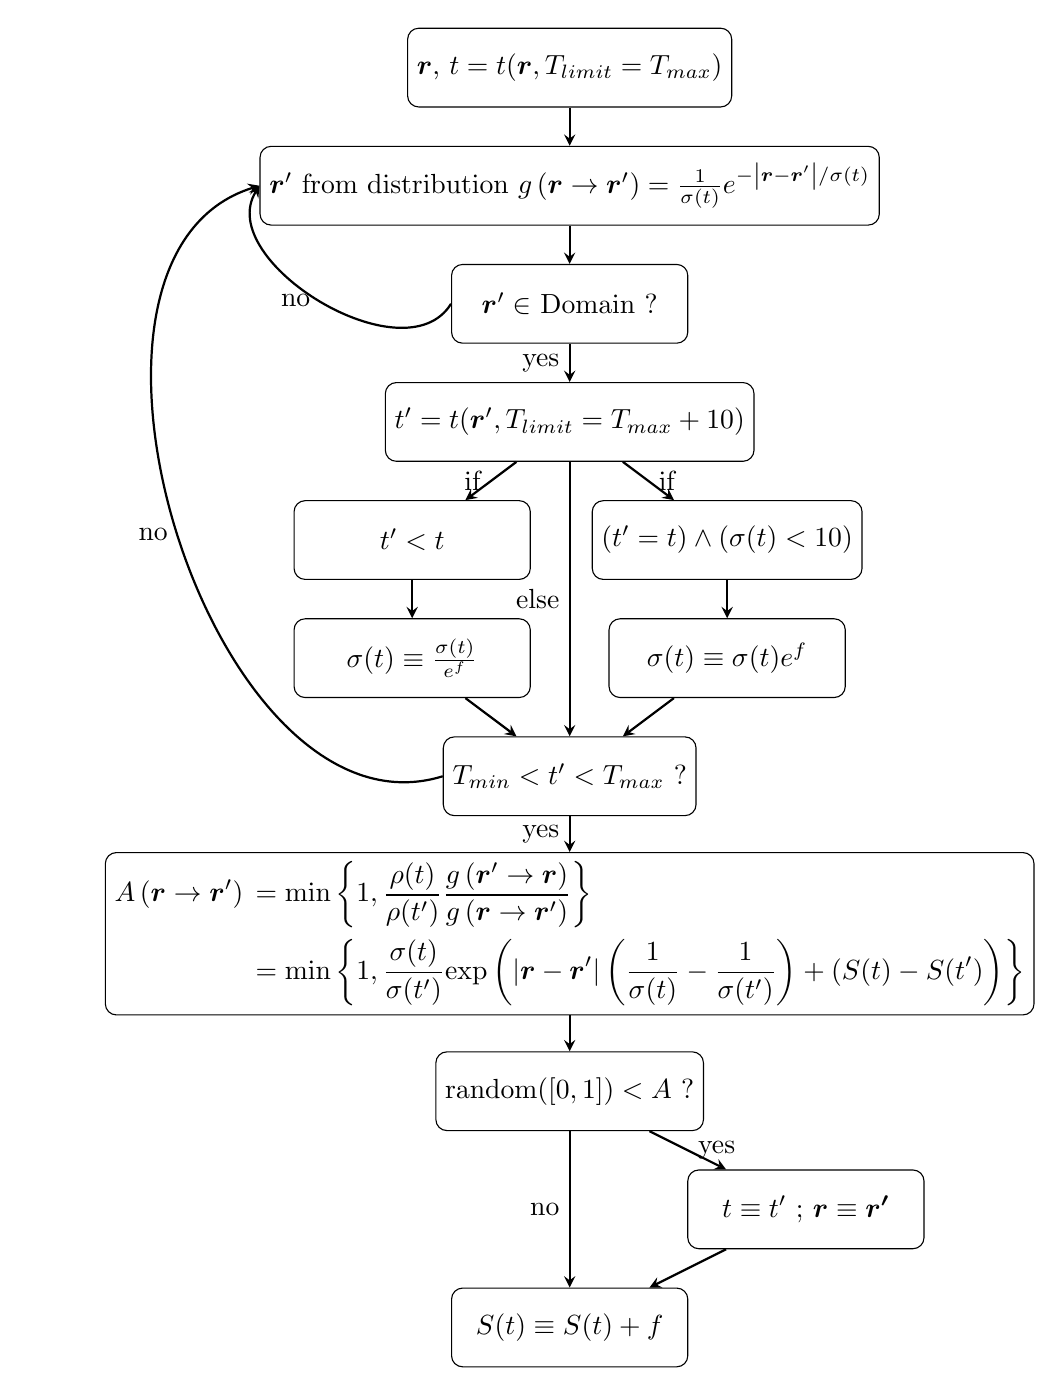
\begin{tikzpicture}[node distance=1.5cm, bend angle=90] 

\node (start) [startstop] {$\boldsymbol{r}$, $t = t(\boldsymbol{r}, T_{limit}=T_{max})$};

\node (g) [startstop, below of=start] {$\boldsymbol{r}^{\prime}$ from distribution  $g\left(\boldsymbol{r} \rightarrow \boldsymbol{r}^{\prime}\right)=\frac{1}{\sigma(t)} e^{-\left|\boldsymbol{r}-\boldsymbol{r}^{\prime}\right| / \sigma(t)}$};

\node (box) [startstop, below of=g] {$\boldsymbol{r}^{\prime} \in$ Domain ?};

\node(tline) [startstop, below of=box] {$t^{\prime} = t(\boldsymbol{r}^{\prime}, T_{limit}=T_{max}+10)$};

\node(less) [startstop, below of=tline, xshift=-2cm]  {$t^{\prime} < t$};
\node(cless)[startstop, below of=less] {$\sigma(t) \equiv \frac{\sigma(t)}{e^f}$};

\node(more) [startstop, below of=tline, xshift=2cm]  {$(t^{\prime} = t) \land (\sigma(t) < 10)$};
\node(cmore)[startstop, below of=more] {$\sigma(t) \equiv \sigma(t)e^f$};

\node(tbox) [startstop, below of=cless, xshift=2cm] {$T_{min} < t^{\prime} < T_{max}$ ?};

\node(a) [startstop, below of=tbox, yshift = -0.5cm] {
$\begin{aligned} 
A\left(\boldsymbol{r} \rightarrow \boldsymbol{r}^{\prime}\right){} 
& =\min \left\{1, \frac{\rho(t)}{\rho(t^{\prime})} \frac{g\left(\boldsymbol{r}^{\prime} \rightarrow \boldsymbol{r}\right)}{g\left(\boldsymbol{r} \rightarrow \boldsymbol{r}^{\prime}\right)}\right\} \\
& = \min \left\{1, \frac{\sigma(t)}{\sigma(t^{\prime})} \text{exp}\left(\left|\boldsymbol{r}-\boldsymbol{r}^{\prime}\right|   \left(\frac{1}{\sigma(t)}-\frac{1}{\sigma(t^{\prime})}\right)+(S(t)-S(t^{\prime})    \right) \right\}
\end{aligned}$};

\node(rand)[startstop, below of=a, yshift = -0.5cm] {$\text{random}([0,1])< A$ ?};

\node(sub)[startstop, below of=rand, xshift = 3cm]{$t \equiv t^{\prime}$ ; $\boldsymbol{r} \equiv \boldsymbol{r^{\prime}}$};

\node(end)[startstop, below of=sub, xshift = -3cm]{$S(t) \equiv S(t)+f$};

\draw [arrow] (start) -- (g); 
\draw [arrow] (g) -- (box); 
\draw [arrow] (box) -- node[anchor=east] {yes} (tline); 
\draw [arrow] (tline) -- node[anchor=east] {if} (less);
\draw [arrow] (tline) -- node[anchor=west] {if} (more);
\draw [arrow] (tline) -- node[anchor=east] {else} (tbox);
\draw [arrow] (less) -- (cless); 
\draw [arrow] (more) -- (cmore); 
\draw [arrow] (cless) -- (tbox); 
\draw [arrow] (cmore) -- (tbox);
\draw [arrow] (tbox) -- node[anchor=east] {yes} (a);
\draw [arrow] (a) -- (rand);
\draw [arrow] (rand) -- node[anchor=west] {yes} (sub);
\draw [arrow] (rand) -- node[anchor=east] {no} (end);
\draw [arrow] (sub) -- (end);

\draw [arrow] (tbox) edge [bend left] node[anchor=east] {no} (g);
\draw [arrow] (box) edge [bend left] node[anchor=east] {no} (g);

\end{tikzpicture}
\par\end{center}
\end{doublespace}

\newpage{}
\begin{doublespace}
\begin{center}
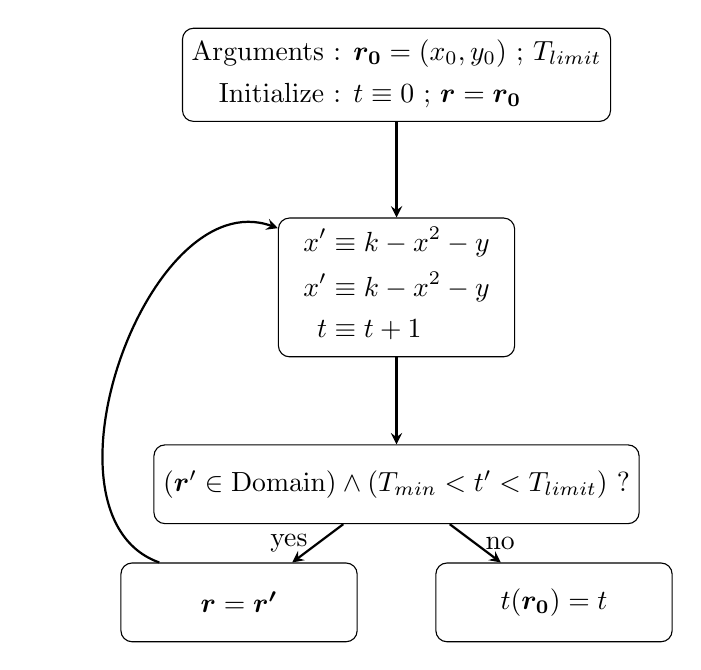
\begin{tikzpicture}[node distance=1.5cm, bend angle=90] 

\node (start) [startstop] 
{$\begin{aligned} 
 \text{Arguments : } & \boldsymbol{r_{0}} = (x_{0},y_{0})\text{ ; } T_{limit} \\
 \text{Initialize : } & t \equiv 0 \text{ ; } \boldsymbol{r} = \boldsymbol{r_{0}}
\end{aligned}$};

\node (map) [startstop, below of=start, yshift = -1.2cm]
{$\begin{aligned} 
 x^{\prime} & \equiv k-x^{2}-y \\
 x^{\prime} & \equiv k-x^{2}-y \\
 t          & \equiv t+1
\end{aligned}$};

\node (box) [startstop, below of=map, yshift=-1cm] 
{($\boldsymbol{r}^{\prime} \in \text{Domain}) \land (T_{min} < t^{\prime} < T_{limit})$ ?};

\node (repeat) [startstop, below of=box, xshift = -2cm]{$\boldsymbol{r} = \boldsymbol{r^{\prime}}$};
\node (end) [startstop, below of=box, xshift = 2cm]{$t(\boldsymbol{r_{0}}) = t$};

\draw [arrow] (start) -- (map);
\draw [arrow] (map) -- (box);
\draw [arrow] (box) -- node[anchor=west] {no} (end);
\draw [arrow] (box) -- node[anchor=east] {yes} (repeat);
\draw [arrow] (repeat) edge [bend left] (map);

\end{tikzpicture}
\par\end{center}
\end{doublespace}

\newpage{}

\subsection{Nelder-Mead Algorithm}

Reference: Gao, F. and Han, L. Implementing the Nelder-Mead simplex
algorithm with adaptive parameters. 2012. Computational Optimization
and Applications. 51:1, pp. 259-277

Let $f:\mathbb{R}^{n}\rightarrow\mathbb{R}$ be the function to be
minimized. A n-dimensional simplex is the convex hull (smallest convex
set) delimited by n+1 points (vertices). Let $\Delta$ denote the
simplex and $\mathbf{x}_{1}$,...,$\mathbf{x}_{n+1}$ the vertices
which define it. The method makes use of the following definitions,
with $\alpha>0$, $\beta>1$, $0<\gamma<1$ and $0<\delta<1$.

\begin{doublespace}
One iteration of the algorithm proceeds as follows:\\

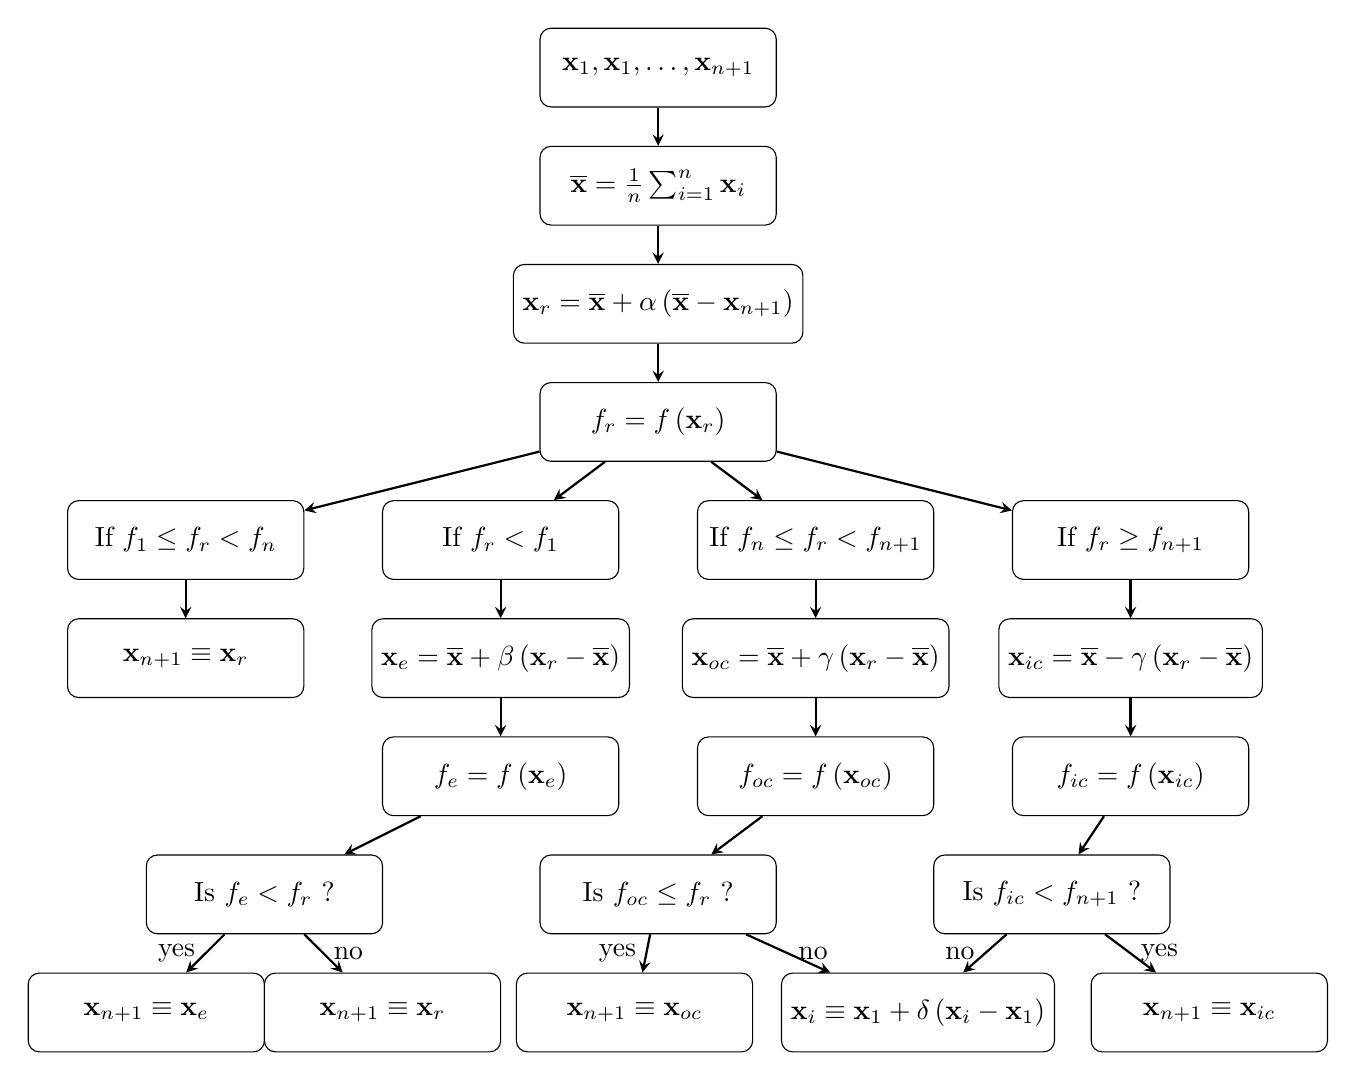
\begin{tikzpicture}[node distance=1.5cm] 
\node (start) [startstop] {$\mathbf{x}_{1}, \mathbf{x}_{1}, \dots, \mathbf{x}_{n+1}$};
\node (centroid) [startstop, below of=start] {$\overline{\mathbf{x}}=\frac{1}{n} \sum_{i=1}^{n} \mathbf{x}_{i}$}; 
\node (r) [startstop, below of=centroid] {$\mathbf{x}_{r}=\overline{\mathbf{x}}+\alpha\left(\overline{\mathbf{x}}-\mathbf{x}_{n+1}\right)$}; 
\draw [arrow] (start) -- (centroid); \draw [arrow] (centroid) -- (r);
\node (fr) [startstop, below of=r] {$f_{r}=f\left(\mathbf{x}_{r}\right)$}; \draw [arrow] (r) -- (fr);
\node (cond1) [startstop, below of=fr, xshift=-6cm] {If $ f_{1} \leq f_{r}<f_{n}$}; 
\node (cond2) [startstop, below of=fr, xshift=-2cm] {If $ f_{r}<f_{1}$}; 
\node (cond3) [startstop, below of=fr, xshift=2cm] {If $ f_{n} \leq f_{r}<f_{n+1}$};
\node (cond4) [startstop, below of=fr, xshift=6cm] {If $ f_{r} \geq f_{n+1}$};

\draw [arrow] (fr) -- (cond1); \draw [arrow] (fr) -- (cond2); \draw [arrow] (fr) -- (cond3); \draw [arrow] (fr) -- (cond4);

\node (endr) [startstop, below of=cond1] {$\mathbf{x}_{n+1}\equiv\mathbf{x}_{r}$}; 
\node (e) [startstop, below of=cond2] {$\mathbf{x}_{e}=\overline{\mathbf{x}}+\beta\left(\mathbf{x}_{r}-\overline{\mathbf{x}}\right)$}; 
\node (oc) [startstop, below of=cond3] {$\mathbf{x}_{o c}=\overline{\mathbf{x}}+\gamma\left(\mathbf{x}_{r}-\overline{\mathbf{x}}\right)$}; 
\node (ic) [startstop, below of=cond4] {$\mathbf{x}_{i c}=\overline{\mathbf{x}}-\gamma\left(\mathbf{x}_{r}-\overline{\mathbf{x}}\right)$}; 

\draw [arrow] (cond1) -- (endr); \draw [arrow] (cond2) -- (e); \draw [arrow] (cond3) -- (oc); \draw [arrow] (cond4) -- (ic);

\node (fe) [startstop, below of=e] {$f_{e}=f\left(\mathbf{x}_{e}\right)$}; 
\node (foc) [startstop, below of=oc] {$f_{o c}=f\left(\mathbf{x}_{o c}\right)$}; 
\node (fic) [startstop, below of=ic] {$f_{i c}=f\left(\mathbf{x}_{i c}\right)$};

\draw [arrow] (e) -- (fe); \draw [arrow] (oc) -- (foc); \draw [arrow] (ic) -- (fic);

\node (conde) [startstop, below of=fe, xshift=-3cm] {Is $f_{e}<f_{r}$ ?}; 
\node (condoc) [startstop, below of=foc, xshift=-2cm] {Is $f_{o c} \leq f_{r}$ ?}; 
\node (condic) [startstop, below of=fic, xshift=-1cm] {Is $f_{i c}<f_{n+1}$ ?}; 

\draw [arrow] (fe) -- (conde); \draw [arrow] (foc) -- (condoc); \draw [arrow] (fic) -- (condic);

\node (ende) [startstop, below of=conde, xshift=-1.5cm] {$\mathbf{x}_{n+1}\equiv\mathbf{x}_{e}$}; 
\node (endr2) [startstop, below of=conde, xshift=1.5cm] {$\mathbf{x}_{n+1}\equiv\mathbf{x}_{r}$};
\node (endoc) [startstop, below of=condoc, xshift=-0.3cm] {$\mathbf{x}_{n+1}\equiv\mathbf{x}_{o c}$};
\node (endic) [startstop, below of=condic, xshift=2cm] {$\mathbf{x}_{n+1}\equiv\mathbf{x}_{i c}$};

\draw [arrow] (conde) -- node[anchor=east] {yes} (ende); \draw [arrow] (conde) -- node[anchor=west] {no} (endr2);
\draw [arrow] (condoc) -- node[anchor=east] {yes} (endoc); \draw [arrow] (condic) -- node[anchor=west] {yes} (endic);

\node (shrink) [startstop, below of=condoc, xshift=3.3cm] {$\mathbf{x}_{i} \equiv \mathbf{x}_{1}+\delta\left(\mathbf{x}_{i}-\mathbf{x}_{1}\right)$};
\draw [arrow] (condoc) -- node[anchor=west] {no} (shrink); \draw [arrow] (condic) -- node[anchor=east] {no} (shrink);

\end{tikzpicture}\\

\end{doublespace}

An optimal choice of initial vertices of the simplex and $\{\alpha,\beta,\gamma,\delta\}$
values is highly dependent on the nature of the problem. Althought
there is no special termination condition associated with the algorithm,
Nelder and Mead used the standard deviation of the values of the function
on the vertices of the simplex. 

\newpage{}

\subsection{Powell's Method}

References: Brent, Richard P. (1973). \textquotedbl Section 7.3:
Powell's algorithm\textquotedbl . Algorithms for minimization without
derivatives; Flannery, BP (2007); Numerical Recipes: The Art of Scientific
Computing.

To understand this method, we must first have the definition of \textit{conjugate}
directions. Consider the following Taylor series approximation to
a function $f(\mathbf{X})$ and a point $\mathbf{P}$:
\begin{center}
$f(\mathbf{x})=f(\mathbf{P})+\sum_{i}\frac{\partial f}{\partial x_{i}}x_{i}+\frac{1}{2}\sum_{i,j}\frac{\partial^{2}f}{\partial x_{i}\partial x_{j}}x_{i}x_{j}+\cdots\approx c-\mathbf{b}\cdot\mathbf{x}+\frac{1}{2}\mathbf{x}\cdot\mathbf{A}\cdot\mathbf{x}$
\par\end{center}

\noindent where
\begin{center}
$c\equiv f(\mathbf{P})\quad\mathbf{b}\equiv-\nabla f\left|\mathbf{P}\quad[\mathbf{A}]_{ij}\equiv\frac{\partial^{2}f}{\partial x_{i}\partial x_{j}}\right|_{\mathbf{P}}$
\par\end{center}

\noindent and the approximation to the functions gradient:
\begin{center}
$\nabla f=\mathbf{A}\cdot\mathbf{x}-\mathbf{b}$
\par\end{center}

Therefore, the gradient will vanish - the function will be at a neighbouring
extremum - at $\mathbf{P+x}$ where $\mathbf{x}$ is the solution
to $\mathbf{A}\cdot\mathbf{x}=\mathbf{b}$. If we move along that
direction to a minimum and now consider moving in a direction $\mathbf{v}$,
in order not to ruin the previous minimization, we pretend that the
gradient continues to be perpendicular to $\mathbf{x}$. Considering
a change in the gradient:
\begin{center}
$\delta(\nabla f)=\mathbf{A}\cdot(\delta\mathbf{v})$
\par\end{center}

we therefore are interested in directions $\mathbf{v}$ that satisfy:
\begin{center}
$0=\mathbf{u}\cdot\delta(\nabla f)=\mathbf{u}\cdot\mathbf{A}\cdot\mathbf{v}$
\par\end{center}

When this equation holds for two directions $\mathbf{u}$ and $\mathbf{v}$,
they are said to be \textit{conjugate}. Powell's method produces
$n$ mutually conjugate directions for an objective $n$-dimensional
function, and needs an 1-dimensional minimization algorithm such as
Golden Search to minimize $f(\mathbf{x})$ in a particular direction.
The initial directions $\mathbf{u}_{0},...,\mathbf{u}_{i+1}$ are
usually chosen to be the cartesian basis vectors. An iteration of
the algorithm is represented below.
\begin{center}
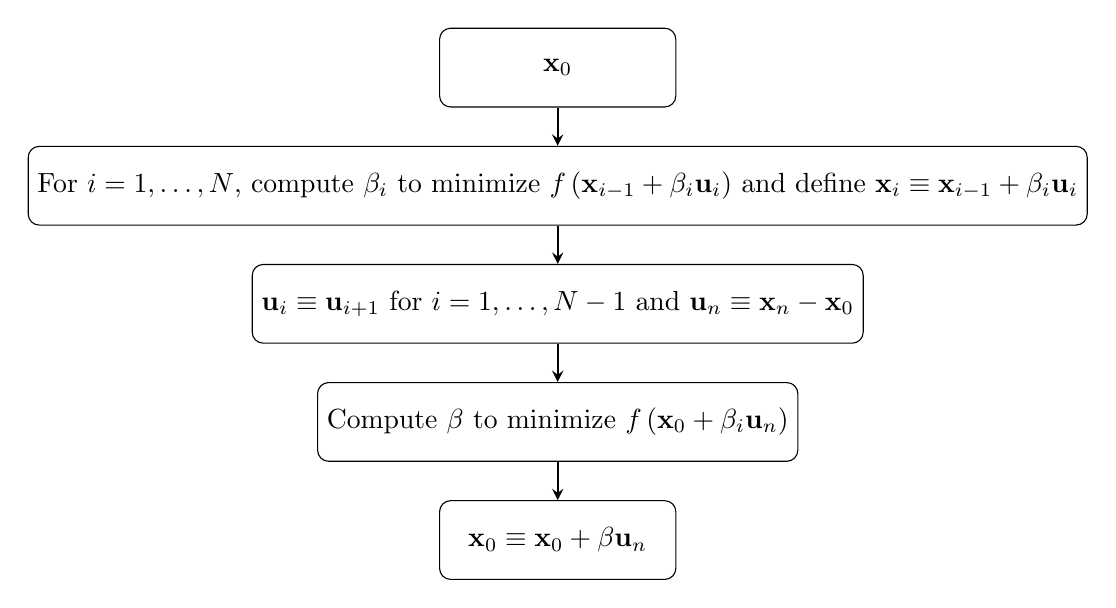
\begin{tikzpicture}[node distance=1.5cm] 
\node (step0) [startstop] {$\mathbf{x}_{0}$};
\node (step1) [startstop, below of=step0] {For $i=1, \dots, N$, compute $\beta_{i}$ to minimize $f\left(\mathbf{x}_{i-1}+\beta_{i} \mathbf{u}_{i}\right)$ and define $\mathbf{x}_{i} \equiv \mathbf{x}_{i-1}+\beta_{i} \mathbf{u}_{i}$};
\node (step3) [startstop, below of=step1] {$\mathbf{u}_{i} \equiv \mathbf{u}_{i+1}$ for $i=1, \dots, N-1 $ and $\mathbf{u}_{n} \equiv \mathbf{x}_{n}-\mathbf{x}_{0}$};
\node (step4) [startstop, below of=step3] {Compute $\beta$ to minimize $f\left(\mathbf{x}_{0}+\beta_{i} \mathbf{u}_{n}\right)$};
\node (step5) [startstop, below of=step4] {$\mathbf{x}_{0} \equiv \mathbf{x}_{0}+\beta \mathbf{u}_{n}$};

\draw [arrow] (step0) -- (step1); \draw [arrow] (step1) -- (step3);
\draw [arrow] (step3) -- (step4); \draw [arrow] (step4) -- (step5);

\end{tikzpicture}
\par\end{center}

\newpage{}

\section{The Rosenbrock function}

\begin{figure}[H]
\begin{centering}
\includegraphics[scale=0.3]{pictures/rosen}
\par\end{centering}
\caption{Rosenbrock function ($z=f(x,y)$) for $a=1\text{ and }b=100$.}

\end{figure}

The Rosenbrock function (represented in the figure above) is a non-convex
function which is used as a performance test problem for optimization
algorithms. The global minimum is inside a long, narrow, parabolic
shaped flat valley, and minimization algorithms usually converge rapidly
to this valley, but converging to the actual global minimum is harder.
The function is defined as:
\begin{center}
$f(x,y)=(a-x)^{2}+b\left(y-x^{2}\right)^{2}$
\par\end{center}

Its partial derivatives are:
\begin{center}
$\frac{\partial f}{\partial x}(x,y)=2(a-x)-4bx(y-x^{2})$
\par\end{center}

\begin{center}
$\frac{\partial f}{\partial y}(x,y)=2b(y-x^{2})$
\par\end{center}

Calculating extremum points:
\begin{center}
$\frac{\partial f}{\partial y}(x,y)=0\implies y=x^{2}$
\par\end{center}

\begin{center}
$(y=x^{2}\land\frac{\partial f}{\partial x}(x,y)=0)\implies(x=a\land y=a^{2})$
\par\end{center}

\begin{center}
$f(a,a^{2})=0$
\par\end{center}

The global minimum is therefore located at $(a,a^{2})$ and its value
is $0$.
\end{document}
